\chapter{Propuesta de soluci�n}\label{c:chapter2}
% History Points by type of functionality
\newcommand{\hpa}{0.4} % for Autenticar
\newcommand{\hpr}{0.2} % for Listar
\newcommand{\hpc}{0.4} % for Crear
\newcommand{\hpu}{0.2} % for Modificar
\newcommand{\hpd}{0.2} % for Eliminar
\newcommand{\hpb}{0.2} % for Buscar
\newcommand{\hpe}{0.6} % for Exportar
\newcommand{\hpg}{0.5} % for Exportar

\section*{Introducci�n del cap�tulo}
 El presente cap�tulo aborda las particularidades del sistema de gesti�n a desarrollar. Para registrar las principales caracter�sticas se hace uso de los \ac{rf} y \ac{rnf}. Estos describen las funcionalidades y atributos de calidad que debe poseer el software. En el cap�tulo \ref{c:chapter1}, se seleccion� la metodolog�a \ac{xp} como gu�a para el desarrollo del software; por lo tanto, se utilizan las \ac{hu} como herramienta para una descripci�n detallada de los \ac{rf} y la confecci�n del plan de iteraciones. Mediante el uso de este �ltimo, se proceder� a la estimaci�n del tiempo requerido para la culminaci�n del desarrollo del sistema y, con el uso de patrones de dise�o, se facilitar� la posterior descripci�n de las tarjetas \ac{crc}.
 
\section{Requisitos}\label{s:req}

\subsection{Requisitos funcionales}
En ingenier�a de software, los \ac{rf} definen un sistema o sus componentes; describen la funci�n que un software debe realizar, ya sean c�lculos, manipulaci�n de datos, procesos de negocios, entre otros.
Ayudan adem�s a capturar los comportamientos planificados para un sistema, este comportamiento puede ser expresado como una funci�n, servicio o tarea que un software debe realizar~\citep{requisitos}. A continuaci�n, se exponen los diferentes \ac{rf} planteados por el usuario:
\begin{RF}
\item Autenticar Usuario
\item Asignar rol a usuario
\\
\item Listar denuncias
\item Crear denuncia
\item Modificar denuncia
\item Eliminar denuncia
\item Buscar denuncia
%\item Exportar listado de denuncias
%\item Imprimir denuncia
%\item Imprimir listado de denuncias
\\
\item Listar resoluciones
\item Crear resoluci�n
\item Modificar resoluci�n
\item Eliminar resoluci�n
\item Exportar resoluci�n
\\
\item Listar comisiones
\item Crear comisi�n
\item Modificar comisi�n
\item Eliminar comisi�n
\item Buscar comisi�n
\\
\item Listar declaraciones
\item Crear declaraci�n
\item Modificar declaraci�n
\item Eliminar declaraci�n
\item Buscar declaraci�n
%\item Exportar declaraci�n
\\
\item Listar casos disciplinarios
\item Crear caso disciplinario
\item Modificar caso disciplinario
\item Buscar caso disciplinario
\\
\item Exportar Resoluci�n de caso
\item Exportar Expediente
\\
\item Listar roles
\item Crear rol
\item Modificar rol
\item Eliminar rol
\item Buscar rol
\end{RF}

\subsection{Requisitos no funcionales}
Los \ac{rnf}, como su nombre sugiere, son aquellos requerimientos que no se refieren directamente a las funciones espec�ficas que proporciona el sistema, sino a las propiedades emergentes de este como la fiabilidad, el tiempo de respuesta y la capacidad de almacenamiento. De forma alternativa definen las restricciones del sistema \citep{sommerville2011software}.\\
Los requisitos no funcionales de la aplicaci�n a desarrollar son:
\\
\noindent Usabilidad:
\begin{RNF}
\item El sistema debe ser una aplicaci�n web
\item La interfaz del sistema debe ser intuitiva y f�cil de usar
\end{RNF}
Hardware y software:
\begin{RNF}[resume]
\item El sistema operativo del servidor debe tener instalado la m�quina virtual de Java 
\item El ordenador donde se ejecute el servidor debe poseer como m�nimo 4GB de \ac{ram} y 10GB de almacenamiento.
\item El cliente del sistema se podr� ejecutar en los principales navegadores web: Google Chrome y navegadores basados en \gls{chromium}, Mozilla Firefox y Safari.
\end{RNF}
Seguridad:
\begin{RNF}[resume]
\item Solo se podr� acceder al sistema despu�s de estar autenticado con usuario y contrase�a v�lidos
\item Solo se podr�n usar las funcionalidades del sistema en dependencia de si el usuario autenticado posee los permisos requeridos para la misma
\end{RNF}
Dise�o e implementaci�n:
\begin{RNF}[resume]
\item Usar JavaScript como lenguaje de programaci�n del lado del cliente.
%\item Usar VueJS como marco de trabajo de desarrollo del lado del cliente.
\item Usar Java como lenguaje de programaci�n del lado del servidor.
\item Usar Spring Boot como \gls{framework} de desarrollo del lado del servidor.

\item Usar la metodolog�a de desarrollo de software \ac{xp}
\end{RNF}
				% Requisitos (En XP no se trabaja con listas de requisitos, sino con HU)
\section{Historias de usuario}
\label{s:hu}
Las HU ser�n representadas mediante tablas divididas por las siguientes secciones:
\begin{description}

	\item [N�mero] Identificador entero incremental en el tiempo;
	\item [Nombre de historia de usuario] Identificador alfanum�rico para su uso
	      entre los desarrolladores y el cliente;
	\item[Usuario] Nombre y apellidos de la persona involucrada en el desarrollo de la \ac{hu};
	\item[Iteraci�n asignada] Identificador entero perteneciente a la iteraci�n en la cual se planea implementar la funcionalidad descrita en la \ac{hu};
	\item[Prioridad en negocio] Las historias de usuarios que describen funcionalidades imprescindibles en el desarrollo del sistema tienen prioridad alta; aquellas que debe tener el sistema, pero que no son necesarias para su funcionamiento, prioridad media; y auxiliares y que son independientes del sistema, prioridad baja.
	\item[Riesgo en desarrollo] Las historias de usuarios que, en caso de tener alg�n error de implementaci�n, puedan afectar la disponibilidad del sistema, tienen un riesgo de desarrollo alto; las \ac{hu} que puedan presentar errores y retrasan la entrega de la versi�n tienen riesgo de desarrollo medio; y las que puedan presentar errores, pero estos son tratados con facilidad y no afectan en desarrollo del proyecto, tienen riesgo de desarrollo bajo.

	\item[Puntos estimados] Tiempo estimado que tardar� el desarrollo de la \ac{hu};
	\item[Descripci�n] Breve descripci�n de \ac{hu};
	\item[Observaciones] Se�alamiento o advertencia del sistema;
	\item[Prototipo de interfaz] Prototipo de interfaz si aplica.
\end{description} \citep{Joskowicz2008}


Los t�tulos de las \ac{hu} generadas son:
\begin{enumerate}[label=HU \arabic*:]

	\item Autenticar Usuario (Prioridad Alta)

	\item Asignar rol a usuario (Prioridad Baja)

	\item Listar denuncias (Prioridad Alta)

	\item Crear una denuncia (Prioridad Alta)

	\item Modificar una denuncia (Prioridad Alta)

	\item Eliminar denuncias (Prioridad Alta)

	\item Buscar denuncias (Prioridad Baja)

	\item Archivar denuncias (Prioridad Alta)

	\item Listar resoluciones decanales (Prioridad Alta)

	\item Crear una resoluci�n decanal (Prioridad Alta)

	\item Modificar una resoluci�n decanal (Prioridad Alta)

	\item Eliminar resoluciones decanales (Prioridad Alta)

	\item Listar comisiones (Prioridad Alta)

	\item Crear comisiones (Prioridad Alta)

	\item Modificar una comisi�n (Prioridad Alta)

	\item Eliminar comisiones (Prioridad Alta)

	\item Buscar comisiones (Prioridad Baja)

	\item Listar declaraciones (Prioridad Alta)

	\item Crear declaraci�n (Prioridad Alta)

	\item Modificar declaraci�n (Prioridad Alta)

	\item Eliminar declaraciones (Prioridad Alta)

	\item Buscar declaraci�n (Prioridad Baja)

	\item Crear caso disciplinario (Prioridad Alta)

	\item Listar casos disciplinarios (Prioridad Alta)

	\item Modificar caso disciplinario (Prioridad Alta)

	\item Buscar caso disciplinario (Prioridad Baja)

	\item Cerrar caso disciplinario (Prioridad Media)

	\item Listar roles (Prioridad Baja)

	\item Crear roles (Prioridad Baja)

	\item Modificar roles (Prioridad Baja)

	\item Eliminar roles (Prioridad Baja)

	\item Buscar roles (Prioridad Baja)

	\item Exportar resoluciones decanales (Prioridad Baja)

	\item Exportar denuncias (Prioridad Baja)

	\item Exportar declaraciones (Prioridad Baja)

	\item Exportar conclusiones de casos (Prioridad Baja)

	\item Exportar resoluciones de casos (Prioridad Baja)

\end{enumerate}
A continuaci�n se presentan las \ac{hu} con mayor prioridad dentro del negocio, determinadas por el cliente e conjunto con el equipo de desarrollo. El resto se podr�n encontrar en la secci�n de ap�ndices \ref{app:hu}: Historias de Usuario.


\begin{userstory}
	\storyname{ Crear una denuncia }
	\storyuser{ Usuario }
	\storyiter{ 1 }
	\storypriority{ Alta }
	\storyrisk{ Medio }
	\storypoints{ 0.4 }
	\storyprogrammer{ \authorA }
	\storydescription{ Como Usuario quiero crear una denuncia para notificar r�pidamente al decano de una indisciplina cometida por uno o varios estudiantes }
	\storyobservation{ }
	\storyinterface{ 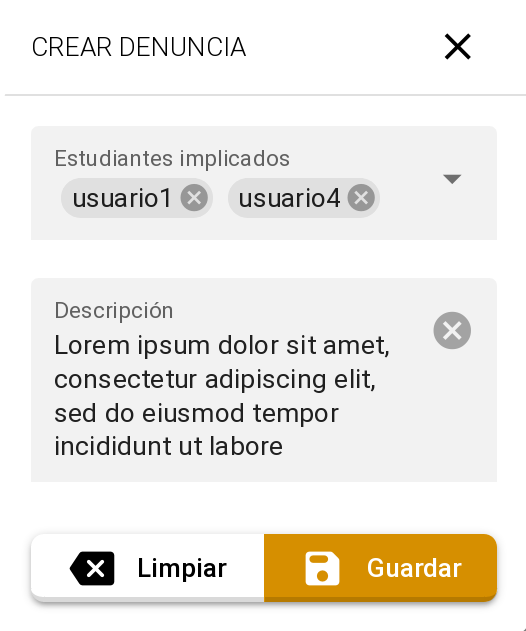
\includegraphics[width=0.5\textwidth]{images/prototypes/cdis-create-denuncia-capture.png} }
\end{userstory}

% Para crear un caso disciplinario basta con asignar una comisi�n a una denuncia pendiente:
% \begin{userstory}
% 	\storyname{ Crear caso disciplinario }
% 	\storyuser{ Decano }
% 	\storyiter{ 1 }
% 	\storypriority{ Alta }
% 	\storyrisk{ Medio }
% 	\storypoints{ 0.4 }
% 	\storyprogrammer{ \authorA }
% 	\storydescription{ Como Decano quiero crear caso disciplinario. }
% 	\storyobservation{ }
% 	\storyinterface{ 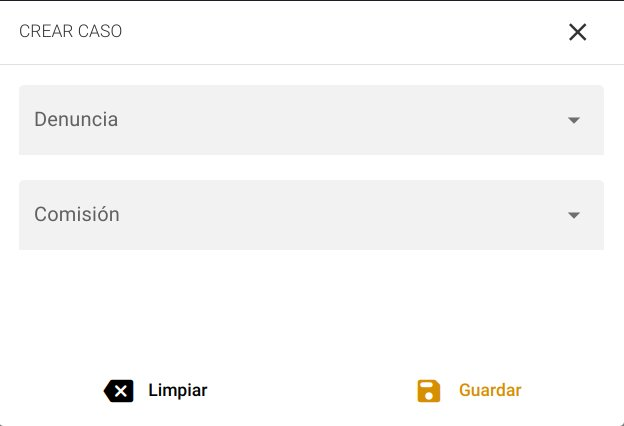
\includegraphics[width=0.5\textwidth]{images/prototypes/cdis-create-caso.png} }
% \end{userstory}					% Historias de usuario
\section{Estimaci�n de esfuerzo por historia de usuario}

\begin {effortestimation}
\addentry[1]{ Listar denuncias }{\hpr}
\addentry[1]{ Crear denuncia }{\hpc}
\addentry[1]{ Modificar denuncia }{\hpu}
\addentry[1]{ Eliminar denuncia }{\hpd}
\addentry[1]{ Buscar denuncia }{\hpb}

\addentry[1]{ Listar comisiones}{\hpr}
\addentry[1]{ Crear comisi�n }{\hpc}
\addentry[1]{ Modificar comisi�n }{\hpc}
\addentry[1]{ Eliminar comisi�n }{\hpc}
\addentry[1]{ Buscar comisi�n }{\hpc}

\addentry[1]{ Listar resoluciones }{\hpr}
\addentry[1]{ Crear resoluci�n }{\hpc}
\addentry[1]{ Modificar resoluci�n }{\hpu}
\addentry[1]{ Eliminar resoluci�n }{\hpd}
\addentry[1]{ Buscar resoluci�n }{\hpb}

\addentry[2]{ Autenticar usuario }{\hpa}

\addentry[2]{ Modificar roles de usuario }{\hpu}
\addentry[2]{ Listar rol}{\hpr}
\addentry[2]{ Crear rol}{\hpc}
\addentry[2]{ Modificar rol}{\hpu}
\addentry[2]{ Eliminar rol}{\hpd}
\addentry[2]{ Buscar rol}{\hpb}

\addentry[3]{ Exportar resoluci�n de caso }{\hpe}
\addentry[3]{ Exportar conclusi�n de la comisi�n }{\hpe}
\end{effortestimation}


	% Estimaci�n de esfuerzo por historia de usuario

\section{Plan de duraci�n de las iteraciones}
\geniterationplan
% Separar generaci�n del plan de iteraciones del siguiente input porque si no no se genera el siguiente input

\section{Tareas de ingenier�a}
La metodolog�a de software XP plantea que la implementaci�n de un software se hace iterativamente.
Durante cada iteraci�n se desarrollan un conjunto de \ac{hu} definidas por el cliente y descritas por el equipo de desarrollo. En esta fase de implementaci�n las \ac{hu} se dividen en tareas, las cuales son asignadas a los programadores para ser implementadas durante la iteraci�n correspondiente \citep{Joskowicz2008}.\\
A continuaci�n, se muestran algunas de las tareas de ingenier�a a realizar por iteraciones.

\subsection{Iteraci�n I}
Para su desarrollo durante la primera iteraci�n se acuerda la selecci�n de las \ac{hu} con mayor prioridad,respetando la opini�n del cliente, cuya suma del tiempo total estimado de desarrollo no exceda el tiempo acordado para las iteraciones ( 2 semanas ). A continuaci�n los nombres de algunas de las \ac{hu} seleccionadas para la realizar las tareas de la primera iteraci�n, una vez implementadas satisfactoriamente, dan paso a la realizaci�n de las pruebas de aceptaci�n:

\begin{itemize}
   \item \textbf{HU3:} Listar denuncias
   \item \textbf{HU4:} Crear una denuncia
   \item \textbf{HU5:} Modificar una denuncia
   \item \textbf{HU6:} Eliminar denuncias
   \item \textbf{HU8:} Archivar denuncias
   \item \textbf{HU9:} Listar resoluciones decanales
   \item \textbf{HU10:} Crear una resoluci�n decanal
   \item \textbf{HU11:} Modificar una resoluci�n decanal
   \item \textbf{HU12:} Listar comisiones
   \item \textbf{HU13:} Crear comisiones
   \item \textbf{HU14:} Modificar una comisi�n
   \item \textbf{HU15:} Eliminar comisiones
   \item \textbf{HU17:} Listar declaraciones
   \item \textbf{HU18:} Crear declaraci�n
   \item \textbf{HU19:} Modificar declaraci�n
   \item \textbf{HU20:} Eliminar declaraciones
   \item \textbf{HU22:} Crear caso disciplinario
   \item \textbf{HU23:} Listar casos disciplinarios
   \item \textbf{HU24:} Modificar caso disciplinario
\end{itemize}




\subsection{Iteraci�n II}
Para su desarrollo durante la segunda iteraci�n se acuerda la selecci�n de las \ac{hu} con prioridad de segundo orden,respetando la opini�n del cliente, cuyo cantidad no exceda la el n�mero de \ac{hu} que se pudieron desarrollar y probar exitosamente en la iteraci�n anterior, lo que se conoce como velocidad de desarrollo. Luego se verifica que las cantidad de tareas total asociadas a las \ac{hu} no excede tampoco la velocidad de desarrollo de la iteraci�n anterior. Y de esta manera se procede con todas las iteraciones siguientes. A continuaci�n los nombres de algunas de las \ac{hu} seleccionadas para realizar las tareas de la segunda iteraci�n, una vez implementadas satisfactoriamente, dan paso a la realizaci�n de las pruebas de aceptaci�n:

\begin{itemize}
   \item \textbf{HU1:} Autenticar Usuario
   \item \textbf{HU2:} Asignar rol a usuario
   \item \textbf{HU7:} Buscar denuncias
   \item \textbf{HU16:} Buscar comisiones
   \item \textbf{HU21:} Buscar declaraci�n
   \item \textbf{HU25:} Buscar caso disciplinario
   \item \textbf{HU27:} Listar roles
   \item \textbf{HU28:} Crear roles
   \item \textbf{HU29:} Modificar roles
   \item \textbf{HU30:} Eliminar roles
   \item \textbf{HU31:} Buscar roles
\end{itemize}

%\begin{table}[]
%\centering
%\begin{tabular}{|ll|lll}
%\cline{1-2}
%\multicolumn{2}{|l|}{Tarea}                                                      &  &  &  \\ \cline{1-2}
%\multicolumn{1}{|l|}{N�mero de tarea: 1}          & N�mero de Historia de usuario: 2 &  &  &  \\ \cline{1-2}
%\multicolumn{2}{|l|}{Nombre de la tarea: Autenticar usuario}                                        &  &  &  \\ \cline{1-2}
%\multicolumn{1}{|l|}{Tipo de tarea: Desarrollo} & Puntos estimados: 1            &  &  &  \\ \cline{1-2}
%\multicolumn{1}{|l|}{Fecha de inicio: 16 de septiembre de 2022}          & Fecha de fin: 17 de septiembre de 2022                 &  &  &  \\ \cline{1-2}
%\multicolumn{2}{|l|}{Programador responsable: \authorA}                                   &  &  &  \\ \cline{1-2}
%\multicolumn{2}{|l|}{Descripci�n: Implementar la autenticaci�n basada en JSON Web Tokens. Deben enviarse en el token los datos del usuario autenticado: Nombre de usuario: String, Nombre: String, Rol: String, Permisos: String[] <[Crear denuncia, Leer denuncia, etc.]>, Cargo: String <Profesor o Decano o Administrador o Estudiante o Trabajador o Secretario de Comunicaci�n de la FEU de la Facultad 4, etc.>}                                                &  &  &  \\ \cline{1-2}
%\end{tabular}
%\end{table}

%\begin{table}[]
%\centering
%\begin{tabular}{|ll|lll}
%\cline{1-2}
%\multicolumn{2}{|l|}{Tarea}                                                      &  &  &  \\ \cline{1-2}
%\multicolumn{1}{|l|}{N�mero de tarea: 1}          & N�mero de Historia de usuario: 2 &  &  &  \\ \cline{1-2}
%\multicolumn{2}{|l|}{Nombre de la tarea: Autenticar usuario}                                        &  &  &  \\ \cline{1-2}
%\multicolumn{1}{|l|}{Tipo de tarea: Desarrollo} & Puntos estimados: 1            &  &  &  \\ \cline{1-2}
%\multicolumn{1}{|l|}{Fecha de inicio: 16 de septiembre de 2022}          & Fecha de fin: 17 de septiembre de 2022                 &  &  &  \\ \cline{1-2}
%\multicolumn{2}{|l|}{Programador responsable: \authorA}                                   &  &  &  \\ \cline{1-2}
%\multicolumn{2}{|l|}{Descripci�n: }                                                &  &  &  \\ \cline{1-2}
%\end{tabular}
%\end{table}
\begin{engineeringtask}[t:engtask1] % label in brackets
   \engtaskuserstory{1}
   \engtaskname{Autenticar usuario}
   \engtasktype{Desarrollo}
   \engtaskpointestimation{1} % d�as ideales de desarrollo
   \engtaskstartdate{16}{9}{2022} % day, month, year
   \engtaskenddate{17}{9}{2022}
   \engtaskprogrammer{\authorA}
   \engtaskdescription{Descripci�n: Implementar la autenticaci�n basada en JSON Web Tokens. Deben enviarse en el token los datos del usuario autenticado:
      Nombre de usuario: String, Nombre: String, Rol: String, Permisos: String[],}

\end{engineeringtask}

\begin{engineeringtask}[t:engtask1.2] % label in brackets
   \engtaskuserstory{1}
   \engtaskname{Manejo de sesi�n}
   \engtasktype{Desarrollo}
   \engtaskpointestimation{1} % d�as ideales de desarrollo
   \engtaskstartdate{17}{9}{2022} % day, month, year
   \engtaskenddate{18}{9}{2022}
   \engtaskdescription{Implementar la persistencia y cierre de sesi�n usando una API web como Local Storage o Cookies para almacenar y recuperar los datos de una sesi�n iniciada, as� como para eliminarlos cuando el usuario decide cerrar la sesi�n.}
   \engtaskprogrammer{\authorA}
\end{engineeringtask}
% \begin{developmenttask}[t:devtask1] % label in brackets
%     \devtaskuserstory{4}
%     \devtaskname{Implementar: Autenticar usuario}
%     \devtasktype{Desarrollo}
%     \devtaskpointestimation{1}
%     \devtaskstartdate{1}{10}{2022} % day, month, year
%     \devtaskenddate{2}{10}{2022}
%     \devtaskdescription{La autenticaci�n debe funcionar usando el servicio de autenticaci�n de la universidad.}
%     \devtaskprogrammer{\authorA}
%  \end{developmenttask}


% \begin{developmenttask}[t:devtask1] % label in brackets
%     \devtaskuserstory{4}
%     \devtaskname{Implementar: Autenticar usuario}
%     \devtasktype{Desarrollo}
%     \devtaskpointestimation{1}
%     \devtaskstartdate{1}{10}{2022} % day, month, year
%     \devtaskenddate{2}{10}{2022}
%     \devtaskdescription{La autenticaci�n debe funcionar usando el servicio de autenticaci�n de la universidad.}
%     \devtaskprogrammer{\authorA}
%  \end{developmenttask}

\subsection{Iteraci�n III}
Para su desarrollo durante la terce iteraci�n se acuerda la selecci�n de las \ac{hu} con prioridad de tercer orden,respetando la opini�n del cliente, cuyo cantidad no exceda la velocidad de desarrollo. Luego se verifica que las cantidad de tareas total asociadas a las \ac{hu} no excede tampoco la velocidad de desarrollo de la iteraci�n anterior. Y de esta manera se procede con todas las iteraciones siguientes. A continuaci�n los nombres de algunas de las \ac{hu} seleccionadas para realizar las tareas de la tercera iteraci�n, una vez implementadas satisfactoriamente, dan paso a la realizaci�n de las pruebas de aceptaci�n:

\begin{itemize}
   \item \textbf{HU26:} Cerrar caso disciplinario
   \item \textbf{HU32:} Exportar resoluciones decanales
   \item \textbf{HU33:} Exportar denuncias
   \item \textbf{HU34:} Exportar declaraciones
   \item \textbf{HU35:} Exportar conclusiones de casos
   \item \textbf{HU36:} Exportar resoluciones de casos
\end{itemize}
\pagebreak
\section{Tarjetas CRC}\label{crc}


\begin{crccard}
   \crcclass{DenunciaController}
   \crcresp{
      \begin{itemize}
         \item crear: Crear una denuncia, la misma se archiva junto con el listado de acusados
         \item listar: Mostrar la denuncia requerida
         \item modificar: Modificar denuncia
         \item borrar: Eliminar denuncia
      \end{itemize}
   }
   \crccolab{
      UsuarioService\\
      DenunciaService\\
      Convertidor\\
      SesionDetails\\
      ValidatorDenuncia\\
      DenunciaUsuarioService\\
      ExpedienteService\\
      CasoUsuarioService\\
      JsonBorrarDenuncia\\
      JsonCrearDenuncia\\
      JsonModificarDenuncia\\
      E\_Denuncia\\
      Mensaje\\
      CasoUsuario\\
      Denuncia\\
      DenunciaUsuario\\
      Usuario\\
   }
\end{crccard}

\begin{crccard}
   \crcclass{ExpedienteController}
   \crcresp{
      \begin{itemize}
         \item listar: Mostrar todos los expedientes de cada estudiante denunciado
         \item modificar: Editar la informaci�n contenida en cada expediente
      \end{itemize}
   }
   \crccolab{
      JsonModificarExpediente\\
      E\_Expediente\\
      ValidatorExpediente\\
      Convertidor\\
      Mensaje\\
      Expediente\\
      ExpedientePK\\
      ExpedienteService\\
   }
\end{crccard}

\begin{crccard}
   \crcclass{ResolucionController}
   \crcresp{
      \begin{itemize}
         \item crear: Crear la resoluci�n con todas las comisiones disciplinarias que conlleva
         \item mostrar: Mostrar todas las resoluciones
         \item borrar: Eliminar una resoluci�n
         \item modificar: Editar una resoluci�n
      \end{itemize}
   }
   \crccolab{
      JsonBorrarResolucion\\
      E\_ExpedienteJsonCrearResolucion\\
      ComisionReducida\\
      JsonModificarResolucion\\
      E\_Resolucion\\
      ValidatorResolucion\\
      Convertidor\\
      Mensaje\\
      Comision\\
      ComisionUsuario\\
      ComisionUsuarioPK\\
      Resolucion\\
      ComisionService\\
      ComisionUsuarioService\\
      ResolucionService\\
      RolService\\
      UsuarioService\\
   }
\end{crccard}
    % Tarjetas CRC
\section{Patrones de dise�o}
Un patr�n de dise�o es una abstracci�n de una soluci�n en un nivel alto. Los patrones solucionan problemas que existen en muchos niveles de abstracci�n. Hay patrones que abarcan las distintas etapas del desarrollo \citep{giraldo2011disenosoft}.

\subsection{Patrones GRASP} Lo esencial de un dise�o de objetos lo constituye el dise�o de las interacciones de objetos y la asignaci�n de responsabilidades. Las decisiones que se tomen pueden influir profundamente en la extensibilidad, claridad y mantenimiento del sistema de software de objetos, adem�s en el grado y calidad de los componentes reutilizables, por esta raz�n, durante el dise�o se deben realizar los casos de usos con objetos basado en los \ac{grasp} \citep{giraldo2011disenosoft}.
Algunos ejemplos de patrones \ac{grasp} utilizados en la implementaci�n de la soluci�n son los siguientes.

\paragraph{Creador:}

Este patr�n implica que un objeto debe responsabilizarse de crear otros:
\begin{itemize}
    \item Si contiene o agrega varios objetos del tipo de los creados.
    \item Si se encarga de registrar objetos del tipo de los creados.
    \item Si utiliza mucho los objetos creados.
    \item O si contiene los datos para crear los del tipo creados.
\end{itemize}

Ejemplo de uso de patr�n creador en la implementaci�n de la propuesta de soluci�n:
\begin{figure}[htp]
    \centering
    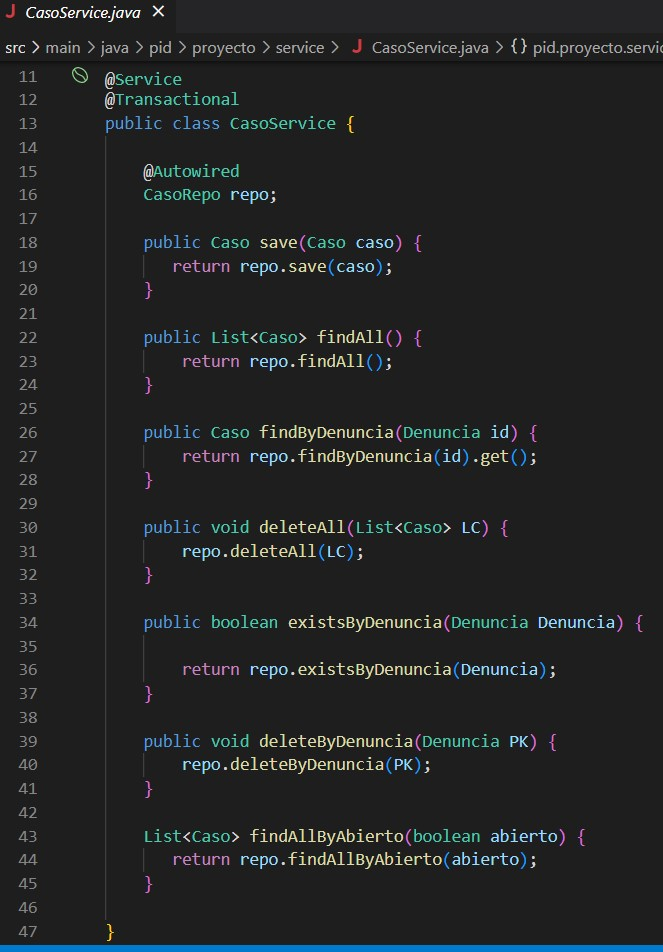
\includegraphics[width=0.6\textwidth]{images/patterns/creator.jpg}
    \caption{Demostraci�n de uso del patr�n controlador}
    \label{fig:creator}
\end{figure}

En la imagen anterior se demuestra el uso del patr�n creador pues la
clase ``CasoService'' hace bastante uso por medio de los m�todos que
dispone de los objetos existentes en la base de datos, hace registros de
los mismos con frecuencia y posee los datos necesarios para crear dichos
objetos.

\paragraph{Controlador \emph{(controller)}:}

Es un patr�n por el cual definimos objetos llamados controladores que
independizan las interfaces con las acciones que haya que hacer.

Estos controladores tienen que ser lo m�s peque�os posible y numerosos,
aislando todo lo posible las capas internas de los programas de las
interfaces.

Ejemplo de uso del patr�n controlador en la implementaci�n de la propuesta de soluci�n: \\
\begin{figure}[htp]
    \centering
    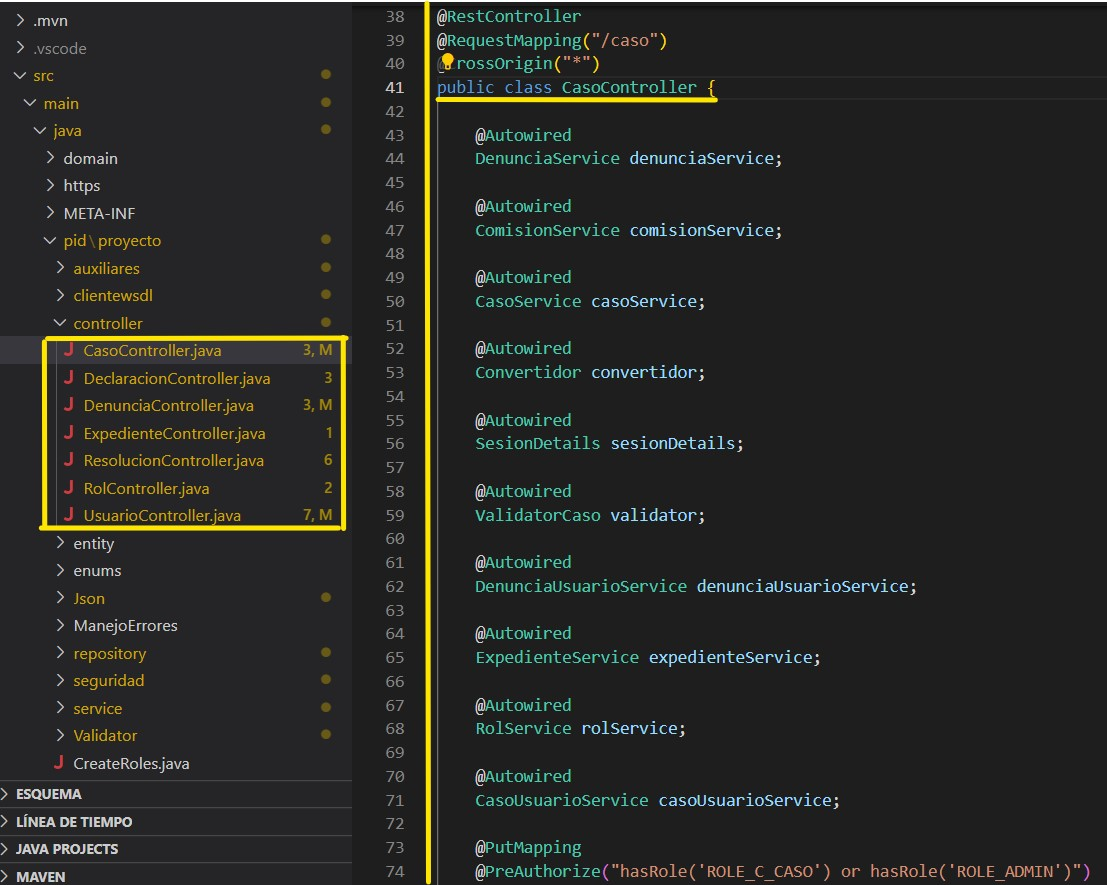
\includegraphics[width=0.6\textwidth]{images/patterns/controller.jpg}
    \caption{Demostraci�n de uso del patr�n controlador}
    \label{fig:controller}
\end{figure}

En la imagen anterior se demuestra el uso del patr�n controlador pues la
clase ``CasoController'', entre otras se�aladas, independizan las
interfaces con acciones que se deben realizar, adem�s de que separan, en la
medida de lo posible, las capas internas de la programaci�n de la
aplicaci�n de su interfaz.




\subsection{Patrones GoF}
En el a�o 1994, apareci� el libro ``Design Patterns: Elements of Reusable Object Oriented Sofware'' escrito por los ahora famosos \emph{Gang of Four} (Pandilla de los cuatro) integrada por Erich Gamma, Richard Helm, Ralph Johnson y John Vlissides. Estos recopilaron y documentaron 23 patrones de dise�o aplicados usualmente por expertos dise�adores de software orientado a objetos. Desde luego ellos no son los inventores ni los �nicos involucrados, pero luego de la publicaci�n de ese libro empez� a difundirse con m�s fuerza la idea de patrones de dise�o. Se distinguen tres tipos de patrones GoF: patrones de comportamiento, patrones creacionales y patrones estructurales \citep{giraldo2011disenosoft}.

\paragraph{�nico \emph{(singleton)}:}
Garantiza que una clase s�lo tenga una instancia, y proporciona un punto de acceso global a ella.\\
\paragraph{ Decorador \emph{(decorator)}:} A�ade funcionalidad a una clase din�micamente. De esta manera, instancias aisladas pueden poseer funcionalidades extra s�lo en tiempo de ejecuci�n.
\paragraph{ Fachada \emph{(facade)}:} Provee de una interfaz unificada simple para acceder a una interfaz o grupo de interfaces de un subsistema.

Ejemplo de uso del patr�n �nico, decorador y fachada en la implementaci�n de la soluci�n:\\

\begin{figure}[h]
    \centering
    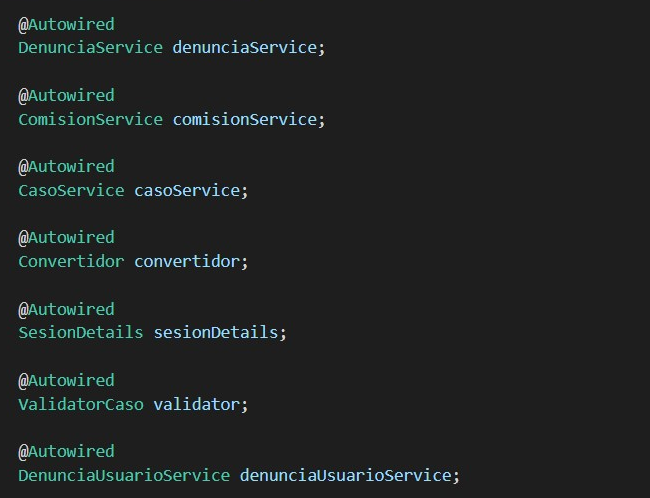
\includegraphics[width=0.6\textwidth]{images/patterns/autowired.png}
    \caption{Demostraci�n de uso del patr�n �nico}
    \label{fig:singleton}
\end{figure}
En la imagen se muestra como se inyecta una instancia �nica de varios objetos que se podr�n usar en una clase controladora para tenerlos como punto de acceso global a ella.
\subsubsection{Patrones creacionales:} Tratan con las formas de crear instancias de objetos. El objetivo de estos patrones es de abstraer el proceso de instanciaci�n y ocultar los detalles de c�mo los objetos son creados o inicializados.
\paragraph{Representante \emph{(proxy)}:} Mantiene un representante de un objeto.
\begin{figure}[htp]
    \centering
    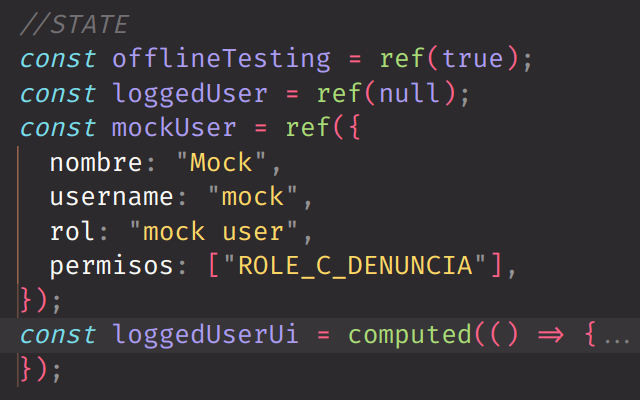
\includegraphics[width=0.8\textwidth]{images/patterns/proxy.png}
    \caption{Uso del patr�n Proxy en la implementaci�n de la soluci�n}
\end{figure}
\subsubsection*{Patrones estructurales:} Describen c�mo clases y objetos pueden ser combinados para formar grandes estructuras y proporcionar nuevas funcionalidades. Estos objetos adicionados pueden ser incluso objetos simples u objetos compuestos.
Proporciona un modo de acceder secuencialmente a los elementos de un objeto agregado sin exponer su representaci�n interna.
Representa y externaliza el estado interno de un objeto sin violar la encapsulaci�n, de forma que �ste puede volver a dicho estado m�s tarde.
\paragraph{ Observador \emph{(observer)}:}  Define una dependencia de uno-a-muchos entre objetos, de forma que cuando un objeto cambie de estado se notifique y actualicen autom�ticamente todos los objetos que dependen de �l.
\begin{figure}[htp]
    \centering
    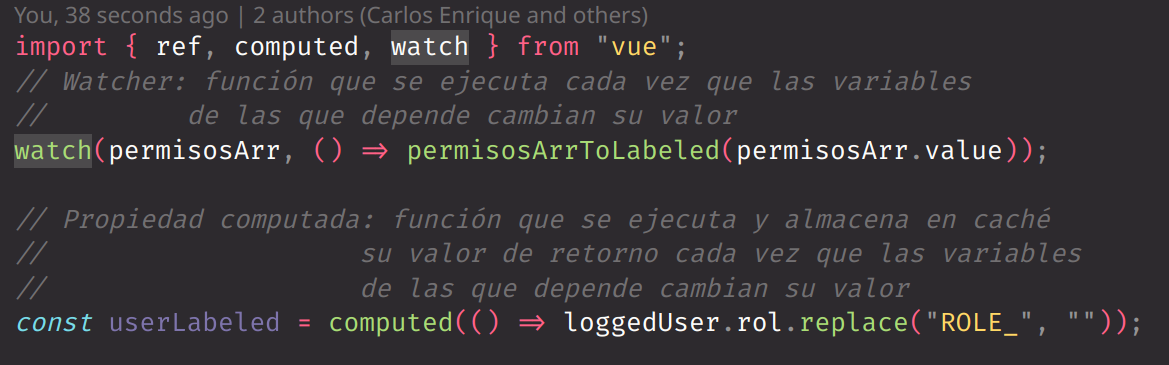
\includegraphics[width=0.8\textwidth]{images/patterns/watch.png}
    \caption{Uso del patr�n Observador en la implementaci�n de la soluci�n}
\end{figure}
\paragraph{ Estado \emph{(state)}:} Permite que un objeto modifique su comportamiento cada vez que cambia su estado interno. Parecer� que cambia la clase del objeto.
       	